% Declare type of document
\documentclass[10pt]{article}

% Import Packages
\usepackage[utf8]{inputenc} 

% Commonly used math symbols and fonts
\usepackage[mathscr]{euscript}
\usepackage{amsfonts,amsmath,amssymb,amsthm}
\usepackage{mathtools,mathdots}

% Better looking default font
\usepackage{lmodern}

% itemize environment
\usepackage{enumitem}

% Array, longtable, and booktabs
\usepackage{array}
\usepackage{longtable}
\usepackage{booktabs}
 
% Caption package for hiding Figure #
\usepackage{caption}

% Page formatting
\usepackage[letterpaper, margin=1in]{geometry}

% Package for nice syntax highlighting for code
% \usepackage[cache=false]{minted}
\usepackage{minted} 

% Allows line breaks in the math environment
\allowdisplaybreaks

\usepackage[activate={true,nocompatibility},final,tracking=true,kerning=true,spacing=true,factor=1100,stretch=10,shrink=10]{microtype}
\microtypecontext{spacing=nonfrench}
% activate={true,nocompatibility} - activate protrusion and expansion
% final - enable microtype; use "draft" to disable
% tracking=true, kerning=true, spacing=true - activate these techniques
% factor=1100 - add 10% to the protrusion amount (default is 1000)
% stretch=10, shrink=10 - reduce stretchability/shrinkability (default is 20/20)


\title{CS 310: Trees (Part I)}
\author{Connor Baker}
\date{February 19, 2019}

\begin{document}

\maketitle

\subsection*{(Rooted) Trees}
\begin{itemize}
    \item A set of nodes and edges with no cycles
    \begin{itemize}
        \item Edges point from parent to child
    \end{itemize}
    \item One special node serves as the root
    \begin{itemize}
        \item There is exactly one incoming edge per node per root
        \item There is a unique path which traverses from the root to each node
    \end{itemize}
\end{itemize}

\subsection*{Examples}
\begin{center}
    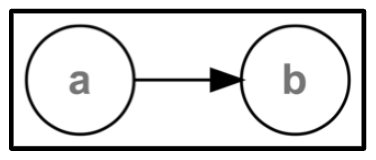
\includegraphics[width = 0.1\textwidth]{images/img00001}
    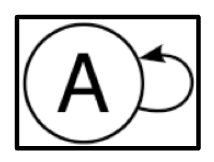
\includegraphics[width = 0.06\textwidth]{images/img00002}
    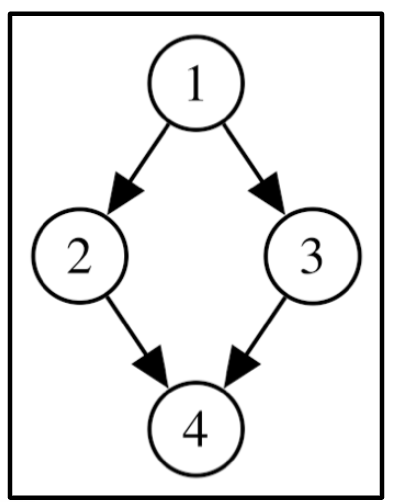
\includegraphics[width = 0.1\textwidth]{images/img00003}
    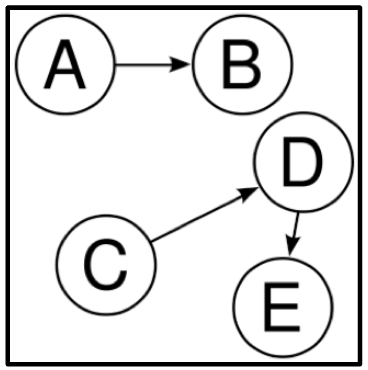
\includegraphics[width = 0.1\textwidth]{images/img00004}
    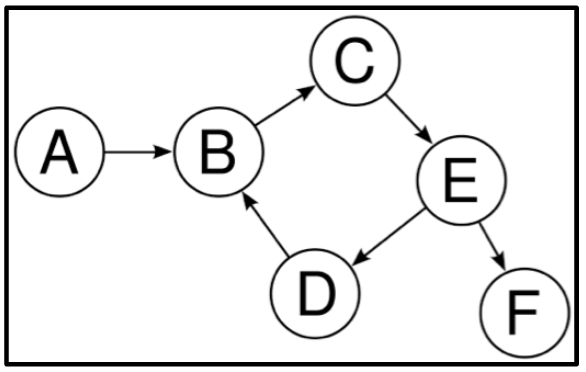
\includegraphics[width = 0.16\textwidth]{images/img00005}
\end{center}
\begin{itemize}
    \item From left to right:
    \begin{itemize}
        \item Tree
        \item Not a tree (it's cyclic)
        \item Not a tree (more than one parent)
        \item Not a tree (disjoint), or two trees, depending on how you look at it
        \item Not a tree (more than one parent)
    \end{itemize}
\end{itemize}

\subsection*{Tree Definitions}
\begin{itemize}
    \item Node relationship:
    \begin{itemize}
        \item The descendants of a node $x$ are all the nodes that we can reach by following the paths starting from $x$ (and sometimes includes the node $x$ itself)
        \item The ancestors of a node $x$ are the nodes on the path from the root to $x$ (and sometimes includes the node $x$ itself)
        \item Nodes are \textit{siblings} if they have the same parent
    \end{itemize}
    \item Special nodes:
    \begin{itemize}
        \item The \textit{root node} is a node that has no parent -- there is only one root node in a rooted tree
        \item A \textit{leaf node} has no children
    \end{itemize}
\end{itemize}

\subsection*{Examples}
\begin{center}
    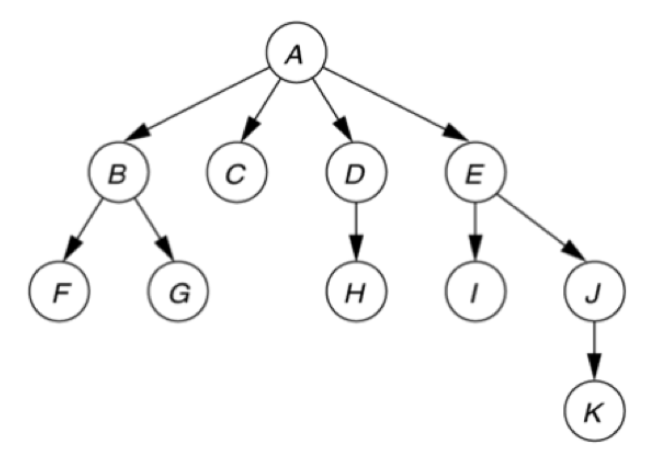
\includegraphics[width = 0.5\textwidth]{images/img00006}
\end{center}
\begin{itemize}
    \item What is the root node?
    \begin{itemize}
        \item $A$
    \end{itemize}
    \item What are the leaf nodes?
    \begin{itemize}
        \item $F,G,C,H,I$ and $K$
    \end{itemize}
    \item What is the parent of $H$?
    \begin{itemize}
        \item $D$
    \end{itemize}
    \item What are the children of $B$?
    \begin{itemize}
        \item $F$ and $G$
    \end{itemize}
    \item What are the ancestors of $G$?
    \begin{itemize}
        \item $B$ and $A$
    \end{itemize}
    \item What are the descendants of $E$?
    \begin{itemize}
        \item $I,J$, and $K$
    \end{itemize}
    \item What are the siblings of $C$?
    \begin{itemize}
        \item $B,D$, and $E$
    \end{itemize}
\end{itemize}

\subsection*{Tree Properties}
\begin{itemize}
    \item Size (the number of nodes)
    \item Node height (the number of levels)
    \begin{itemize}
        \item The \textit{node height} is the length of the path (number of edges) from the node to the deepest leaf
        \item The \textit{tree height} is the height of the root
    \end{itemize}
    \item Node depth (distance from the root)
    \begin{itemize}
        \item The \textit{depth} of a node is the length of the path from the root to the node
    \end{itemize}
\end{itemize}

\subsection*{Example}
\begin{center}
    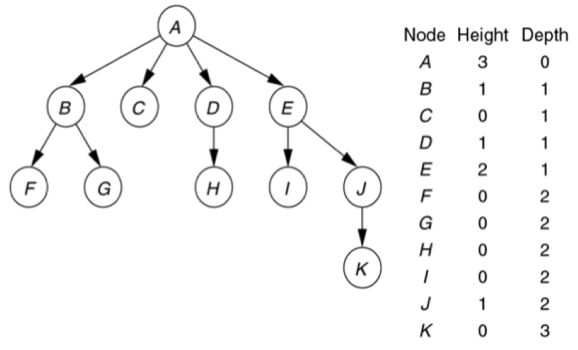
\includegraphics[width = 0.5\textwidth]{images/img00007}    
\end{center}

\subsection*{Tree Features}
\begin{itemize}
    \item Balanced tree
    \begin{itemize}
        \item For a binary tree, the height of the left and right sub-trees of every node differ by 1 or 0 (as used by an AVL tree)
    \end{itemize}
    \item Full tree
    \begin{itemize}
        \item Every node other than the leaves has the maximum number of children
    \end{itemize}
    \item Perfect tree
    \begin{itemize}
        \item A full tree in which all leaves have the same depth
    \end{itemize}
    \item Complete tree (an almost perfect tree)
    \begin{itemize}
        \item A tree that is completely filled, with the possible exception of the bottom level, which is filled from left to right and has no missing nodes
    \end{itemize}
\end{itemize}

\subsection*{Examples (Binary Trees)}
\begin{center}
    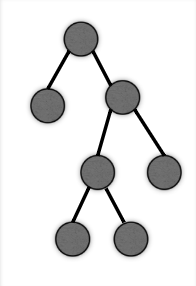
\includegraphics[width = 0.1\textwidth]{images/img00008}
    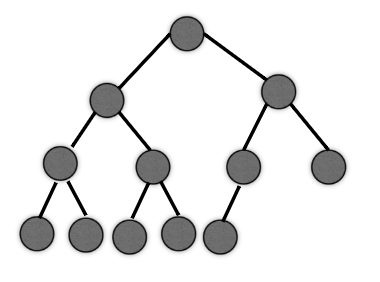
\includegraphics[width = 0.2\textwidth]{images/img00009}
\end{center}
\begin{itemize}
    \item Left: a full tree
    \item Right: a balanced and (nearly) complete tree
\end{itemize}


\subsection*{Trees Implemented with Linked Nodes}
\begin{center}
    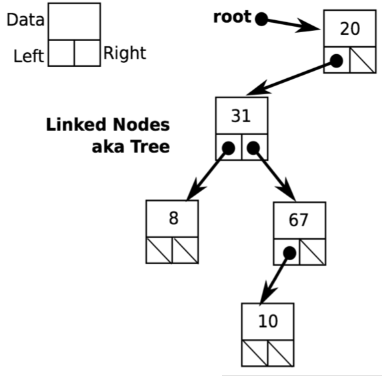
\includegraphics[width = 0.4\textwidth]{images/img00010}
\end{center}
\begin{itemize}
    \item Node structures are typically used for linked lists (owing to the singly-linked \texttt{next}/\texttt{data} idea)
    \item Trees also use nodes
    \begin{itemize}
        \item Data, pointers to children, possibly pointers to parents
        \item Binary trees have left and right children:
        \begin{minted}{java}
class Node<T> {
    T data;
    Node<T> left, right;
}
        \end{minted}
    \end{itemize}
    \item Trees must have a finite number of children -- however, the maximum number of children is arbitrary
\end{itemize}

\section*{Trees Implemented with Arrays}
\begin{itemize}
    \item Store nodes in an array in level order
    \begin{itemize}
        \item Start with the root
        \item Left to right for each level
        \item Reserve space for missing nodes
    \end{itemize}
    \item Used to represent $k$-ary tree
    \begin{itemize}
        \item Each parent can have at most $k$ children
        \item Binary tree when $k=2$
    \end{itemize}
    \item Works the best with trees of a regular structures
    \begin{itemize}
        \item Trees that are perfect or complete don't have (or have small) gaps
        \item There's less wasted memory then
    \end{itemize}
\end{itemize}

\subsection*{Binary Tree with an Array}
\begin{center}
    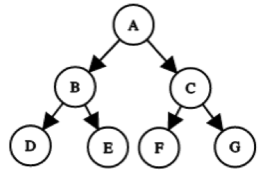
\includegraphics[width = 0.3\textwidth]{images/img00011}

    \begin{tabular}{@{}ccccccc@{}}\hline
    $|$ A $|$&$|$ B $|$&$|$ C $|$&$|$ D $|$&$|$ E $|$&$|$ F $|$&$|$ G $|$\\ \hline
    0 & 1 & 2 & 3 & 4 & 5 & 6 \\
    \end{tabular}
\end{center}
\begin{itemize}
    \item Root is at index 0
    \item Parent at index $p$:
    \begin{itemize}
        \item Left child: $2p+1$
        \item Right child: $2p+2$
    \end{itemize}
    \item Child at index $c$:
    \begin{itemize}
        \item Parent at index $\lfloor (c-1)/2 \rfloor$
    \end{itemize}
\end{itemize}

\subsection*{Binary Tree with an Array}
\begin{itemize}
    \item Complete binary trees
    \begin{itemize}
        \item The array is filled left to right
    \end{itemize}
    \item Arbitrary binary trees
    \begin{itemize}
        \item Some elements of the array can be \mintinline{java}{null}
    \end{itemize}
\end{itemize}

\subsection*{Tree Implementations}
\begin{itemize}
    \item Arrays
    \begin{itemize}
        \item Fast memory access
        \item Must have a fixed branching factor
        \item Inefficient use of memory
        \item Common for regular and stable structures like complete binary trees
    \end{itemize}
    \item Linked nodes
    \begin{itemize}
        \item Easy to move around
        \item Easier to deal with arbitrary trees
    \end{itemize}
\end{itemize}

\subsection*{Tree Applications}
\begin{itemize}
    \item Model hierarchical structures
    \begin{itemize}
        \item File systems, class inheritance
    \end{itemize}
    \item Store sorted data and support efficient search and insertion
    \begin{itemize}
        \item Search trees or ordered trees in $O(\log (n))$ time
        \item Sorted lists and hash tables also come into play
    \end{itemize}
    \item Many others
    \begin{itemize}
        \item Expression trees
        \item Huffman coding
    \end{itemize}
\end{itemize}

\subsection*{Common Tree Operations}
\begin{itemize}
    \item Searching for an item
    \item Adding items
    \item Deleting items
    \item Balancing
    \item Iterating through the tree
    \begin{itemize}
        \item Selecting part of the tree
    \end{itemize}
\end{itemize}

\subsection*{Recursion}
\begin{itemize}
    \item \textit{Recursion}: something defined in terms of itself
    \item \textit{Function recursion}: when a function invokes itself
    \begin{itemize}
        \item Two types of function recursion:
        \begin{itemize}
            \item Direct: a function invokes itself
            \item Indirect: \mintinline{java}{foo} invokes \mintinline{java}{bar}, and \mintinline{java}{bar} invokes \mintinline{java}{foo}
        \end{itemize}
    \end{itemize}
\end{itemize}

\subsection*{Example: Factorial}
\begin{itemize}
    \item Mathematically:
\end{itemize}
$$
n! = \begin{cases}
    1 & n \leq 1 \\
    (n-1)! & n > 1
\end{cases}
$$
\begin{itemize}
\item Programatically:
\begin{minted}{java}
public static int factorial(int n) {
    return (n <= 1) ? 1 : n * factorial(n - 1);
}
\end{minted}
\end{itemize}

\subsection*{Recursion Basics}
\begin{itemize}
    \item Think of your task in terms of a ``base case'' and a ``recursive case''
    \item The \textit{base case} is the answer which is directly calculated with no recursion
    \item The \textit{recursive case} is the answer to be calculated by repeated application
    \begin{itemize}
        \item It is crucial that repeated application of the definition make progress towards the base case
    \end{itemize}
\end{itemize}

\subsection*{Recursive Function Execution}
\begin{center}
    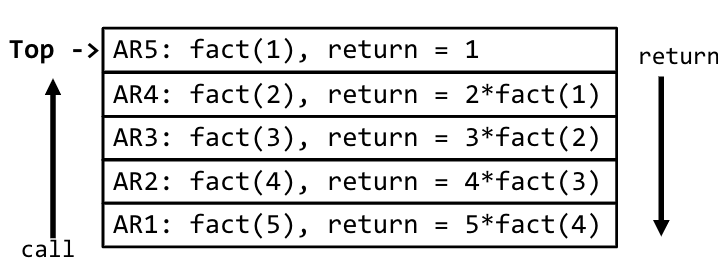
\includegraphics[width = 0.5\textwidth]{images/img00012}
\end{center}
\begin{itemize}
    \item Each recursive call is distinct
    \begin{itemize}
        \item There is a separate frame or activation record on the runtime stack for each call
        \item It's as if they're separate functions with the same implementation
    \end{itemize}
\end{itemize}

\subsection*{Common Issues with Recursion}
\begin{itemize}
    \item The base case is unreachable
    \begin{itemize}
        \item If the recursive definition never triggers the base case, it will never stop
        \item Don't put the base case after the recursive call -- it'll never be reached
    \end{itemize}
    \item The recursive case doesn't make progress towards the base case
    \item Space or time efficiency matters
\end{itemize}

\subsection*{Example}
\begin{itemize}
    \item Consider the following definition of the Fibonacci numbers
\begin{minted}{java}
    public static int fib(int n) {
        return (n <= 2) ? 1 : fib(n - 1) + fib(n - 2);
    }
\end{minted}
    \item For a call to \mintinline{java}{fib(5)}, how many additional calls are made?
    \begin{itemize}
        \item Nine calls
        \item It's $O(2^n)$
    \end{itemize}
\end{itemize}


\end{document}